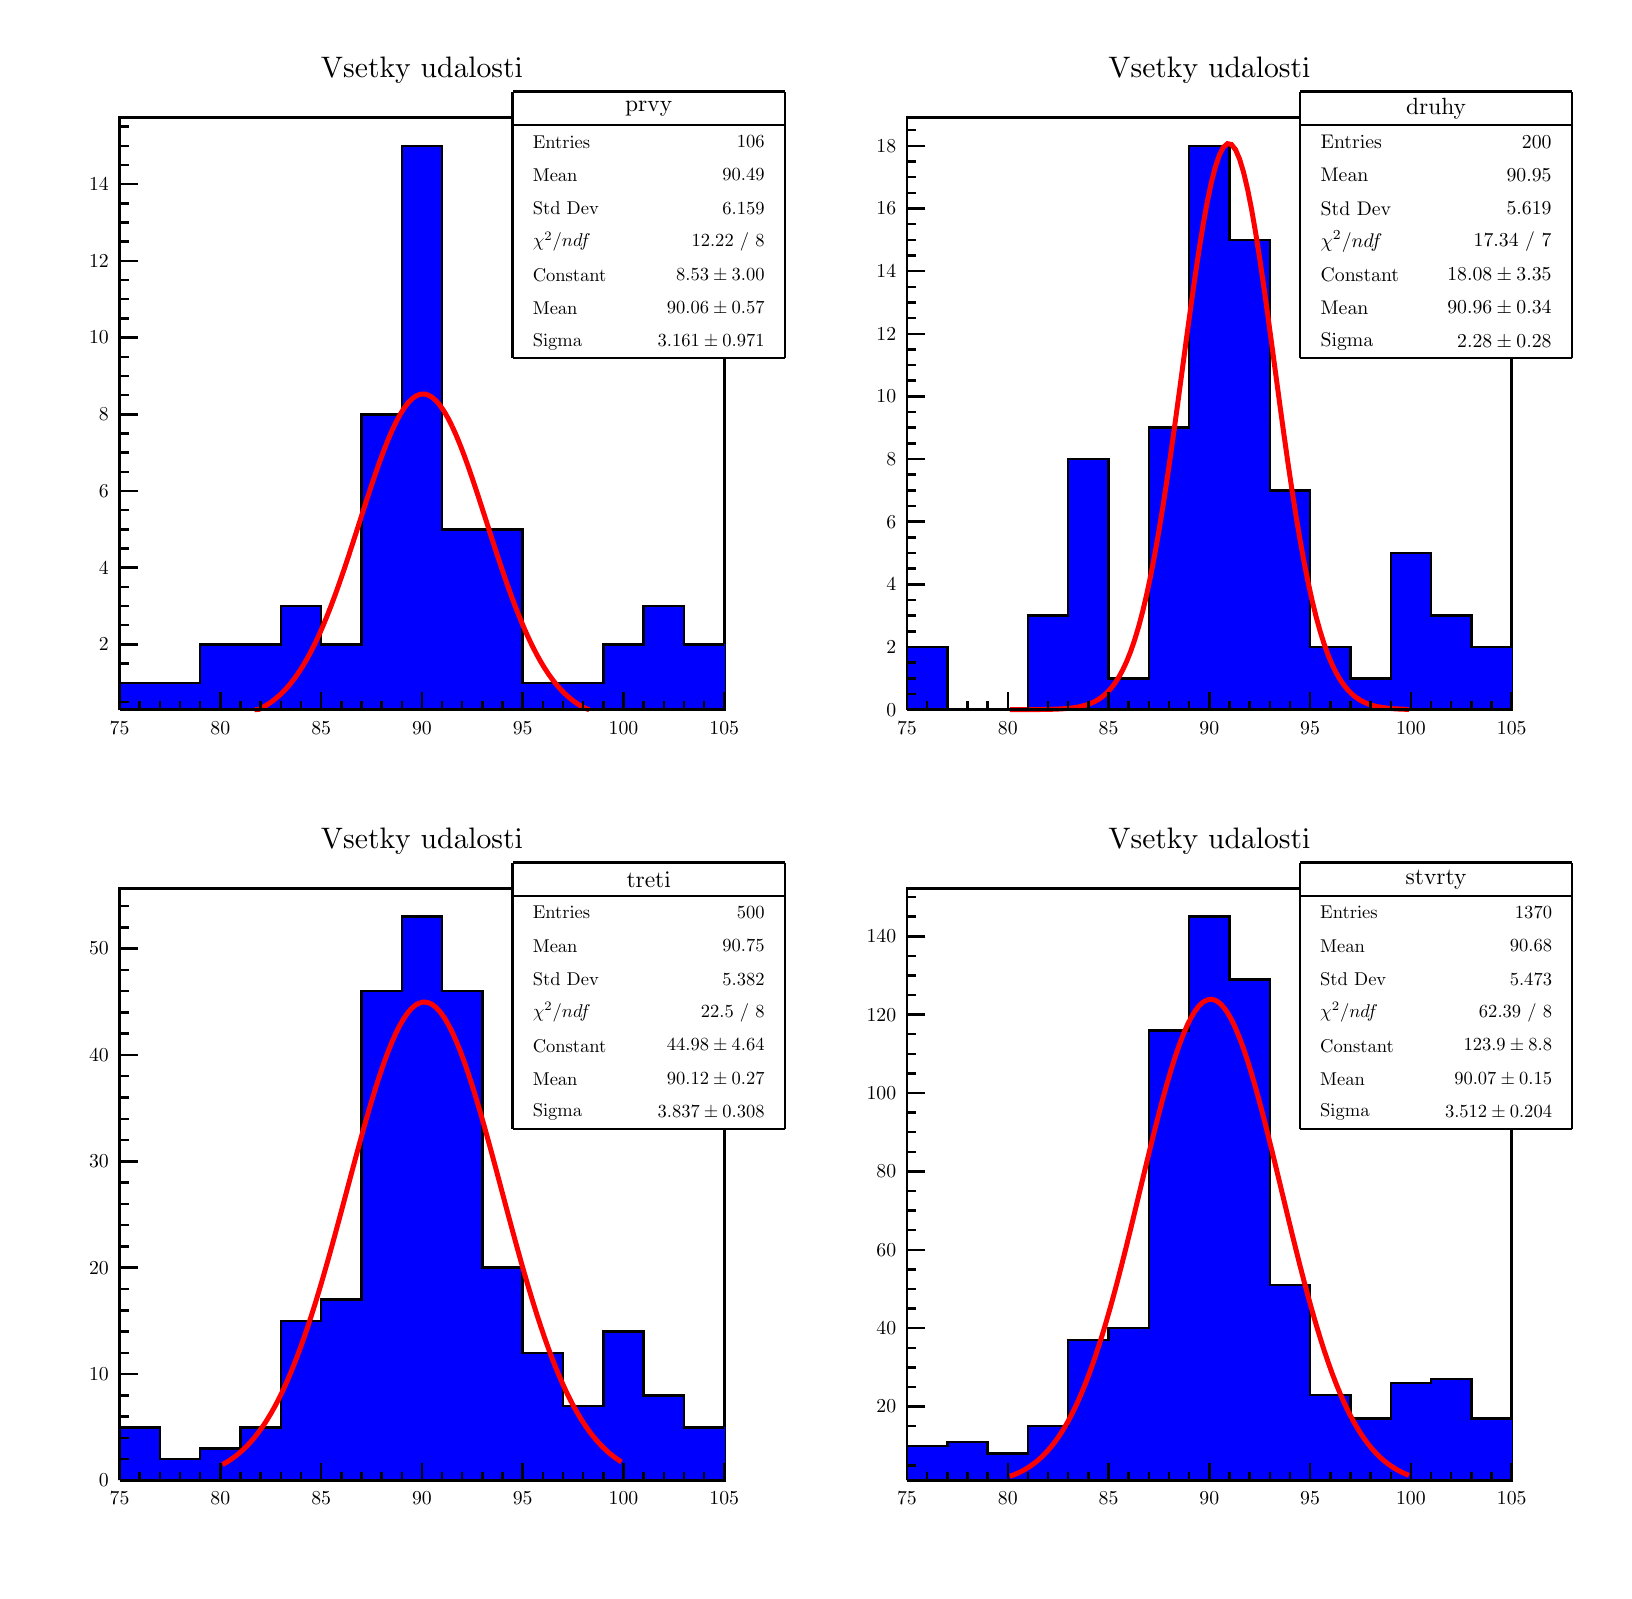
\begin{tikzpicture}
\pgfdeclareplotmark{cross} {
\pgfpathmoveto{\pgfpoint{-0.3\pgfplotmarksize}{\pgfplotmarksize}}
\pgfpathlineto{\pgfpoint{+0.3\pgfplotmarksize}{\pgfplotmarksize}}
\pgfpathlineto{\pgfpoint{+0.3\pgfplotmarksize}{0.3\pgfplotmarksize}}
\pgfpathlineto{\pgfpoint{+1\pgfplotmarksize}{0.3\pgfplotmarksize}}
\pgfpathlineto{\pgfpoint{+1\pgfplotmarksize}{-0.3\pgfplotmarksize}}
\pgfpathlineto{\pgfpoint{+0.3\pgfplotmarksize}{-0.3\pgfplotmarksize}}
\pgfpathlineto{\pgfpoint{+0.3\pgfplotmarksize}{-1.\pgfplotmarksize}}
\pgfpathlineto{\pgfpoint{-0.3\pgfplotmarksize}{-1.\pgfplotmarksize}}
\pgfpathlineto{\pgfpoint{-0.3\pgfplotmarksize}{-0.3\pgfplotmarksize}}
\pgfpathlineto{\pgfpoint{-1.\pgfplotmarksize}{-0.3\pgfplotmarksize}}
\pgfpathlineto{\pgfpoint{-1.\pgfplotmarksize}{0.3\pgfplotmarksize}}
\pgfpathlineto{\pgfpoint{-0.3\pgfplotmarksize}{0.3\pgfplotmarksize}}
\pgfpathclose
\pgfusepathqstroke
}
\pgfdeclareplotmark{cross*} {
\pgfpathmoveto{\pgfpoint{-0.3\pgfplotmarksize}{\pgfplotmarksize}}
\pgfpathlineto{\pgfpoint{+0.3\pgfplotmarksize}{\pgfplotmarksize}}
\pgfpathlineto{\pgfpoint{+0.3\pgfplotmarksize}{0.3\pgfplotmarksize}}
\pgfpathlineto{\pgfpoint{+1\pgfplotmarksize}{0.3\pgfplotmarksize}}
\pgfpathlineto{\pgfpoint{+1\pgfplotmarksize}{-0.3\pgfplotmarksize}}
\pgfpathlineto{\pgfpoint{+0.3\pgfplotmarksize}{-0.3\pgfplotmarksize}}
\pgfpathlineto{\pgfpoint{+0.3\pgfplotmarksize}{-1.\pgfplotmarksize}}
\pgfpathlineto{\pgfpoint{-0.3\pgfplotmarksize}{-1.\pgfplotmarksize}}
\pgfpathlineto{\pgfpoint{-0.3\pgfplotmarksize}{-0.3\pgfplotmarksize}}
\pgfpathlineto{\pgfpoint{-1.\pgfplotmarksize}{-0.3\pgfplotmarksize}}
\pgfpathlineto{\pgfpoint{-1.\pgfplotmarksize}{0.3\pgfplotmarksize}}
\pgfpathlineto{\pgfpoint{-0.3\pgfplotmarksize}{0.3\pgfplotmarksize}}
\pgfpathclose
\pgfusepathqfillstroke
}
\pgfdeclareplotmark{newstar} {
\pgfpathmoveto{\pgfqpoint{0pt}{\pgfplotmarksize}}
\pgfpathlineto{\pgfqpointpolar{44}{0.5\pgfplotmarksize}}
\pgfpathlineto{\pgfqpointpolar{18}{\pgfplotmarksize}}
\pgfpathlineto{\pgfqpointpolar{-20}{0.5\pgfplotmarksize}}
\pgfpathlineto{\pgfqpointpolar{-54}{\pgfplotmarksize}}
\pgfpathlineto{\pgfqpointpolar{-90}{0.5\pgfplotmarksize}}
\pgfpathlineto{\pgfqpointpolar{234}{\pgfplotmarksize}}
\pgfpathlineto{\pgfqpointpolar{198}{0.5\pgfplotmarksize}}
\pgfpathlineto{\pgfqpointpolar{162}{\pgfplotmarksize}}
\pgfpathlineto{\pgfqpointpolar{134}{0.5\pgfplotmarksize}}
\pgfpathclose
\pgfusepathqstroke
}
\pgfdeclareplotmark{newstar*} {
\pgfpathmoveto{\pgfqpoint{0pt}{\pgfplotmarksize}}
\pgfpathlineto{\pgfqpointpolar{44}{0.5\pgfplotmarksize}}
\pgfpathlineto{\pgfqpointpolar{18}{\pgfplotmarksize}}
\pgfpathlineto{\pgfqpointpolar{-20}{0.5\pgfplotmarksize}}
\pgfpathlineto{\pgfqpointpolar{-54}{\pgfplotmarksize}}
\pgfpathlineto{\pgfqpointpolar{-90}{0.5\pgfplotmarksize}}
\pgfpathlineto{\pgfqpointpolar{234}{\pgfplotmarksize}}
\pgfpathlineto{\pgfqpointpolar{198}{0.5\pgfplotmarksize}}
\pgfpathlineto{\pgfqpointpolar{162}{\pgfplotmarksize}}
\pgfpathlineto{\pgfqpointpolar{134}{0.5\pgfplotmarksize}}
\pgfpathclose
\pgfusepathqfillstroke
}
\definecolor{c}{rgb}{1,1,1};
\draw [color=c, fill=c] (0,0) rectangle (20,19.5792);
\draw [color=c, fill=c] (0.2,9.98537) rectangle (9.8,19.3834);
\draw [color=c, fill=c] (1.16,10.9252) rectangle (8.84,18.4436);
\definecolor{c}{rgb}{0,0,0};
\draw [c,line width=0.9] (1.16,10.9252) -- (1.16,18.4436) -- (8.84,18.4436) -- (8.84,10.9252) -- (1.16,10.9252);
\definecolor{c}{rgb}{1,1,1};
\draw [color=c, fill=c] (1.16,10.9252) rectangle (8.84,18.4436);
\definecolor{c}{rgb}{0,0,0};
\draw [c,line width=0.9] (1.16,10.9252) -- (1.16,18.4436) -- (8.84,18.4436) -- (8.84,10.9252) -- (1.16,10.9252);
\definecolor{c}{rgb}{0,0,1};
\draw [c, fill=c] (1.16,10.9252) -- (1.16,11.2661) -- (1.672,11.2661) -- (1.672,11.2661) -- (2.184,11.2661) -- (2.184,11.7532) -- (2.696,11.7532) -- (2.696,11.7532) -- (3.208,11.7532) -- (3.208,12.2403) -- (3.72,12.2403) -- (3.72,11.7532) --
 (4.232,11.7532) -- (4.232,14.6758) -- (4.744,14.6758) -- (4.744,18.0855) -- (5.256,18.0855) -- (5.256,13.2145) -- (5.768,13.2145) -- (5.768,13.2145) -- (6.28,13.2145) -- (6.28,11.2661) -- (6.792,11.2661) -- (6.792,11.2661) -- (7.304,11.2661) --
 (7.304,11.7532) -- (7.816,11.7532) -- (7.816,12.2403) -- (8.328,12.2403) -- (8.328,11.7532) -- (8.84,11.7532) -- (8.84,10.9252);
\definecolor{c}{rgb}{0,0,0};
\draw [c,line width=0.9] (1.16,11.2661) -- (1.672,11.2661) -- (1.672,11.2661) -- (2.184,11.2661) -- (2.184,11.7532) -- (2.696,11.7532) -- (2.696,11.7532) -- (3.208,11.7532) -- (3.208,12.2403) -- (3.72,12.2403) -- (3.72,11.7532) -- (4.232,11.7532) --
 (4.232,14.6758) -- (4.744,14.6758) -- (4.744,18.0855) -- (5.256,18.0855) -- (5.256,13.2145) -- (5.768,13.2145) -- (5.768,13.2145) -- (6.28,13.2145) -- (6.28,11.2661) -- (6.792,11.2661) -- (6.792,11.2661) -- (7.304,11.2661) -- (7.304,11.7532) --
 (7.816,11.7532) -- (7.816,12.2403) -- (8.328,12.2403) -- (8.328,11.7532) -- (8.84,11.7532);
\definecolor{c}{rgb}{1,0,0};
\draw [c,line width=1.8] (2.8752,10.9252) -- (2.9264,10.9278) -- (2.9776,10.9538) -- (3.0288,10.9836) -- (3.08,11.0175) -- (3.1312,11.0559) -- (3.1824,11.0992) -- (3.2336,11.1478) -- (3.2848,11.202) -- (3.336,11.2623) -- (3.3872,11.329) --
 (3.4384,11.4024) -- (3.4896,11.4827) -- (3.5408,11.5703) -- (3.592,11.6652) -- (3.6432,11.7674) -- (3.6944,11.8771) -- (3.7456,11.9941) -- (3.7968,12.1182) -- (3.848,12.249) -- (3.8992,12.3862) -- (3.9504,12.5292) -- (4.0016,12.6772) --
 (4.0528,12.8296) -- (4.104,12.9854) -- (4.1552,13.1434) -- (4.2064,13.3027) -- (4.2576,13.462) -- (4.3088,13.6199) -- (4.36,13.775) -- (4.4112,13.9261) -- (4.4624,14.0715) -- (4.5136,14.2099) -- (4.5648,14.3398) -- (4.616,14.4598) --
 (4.6672,14.5687) -- (4.7184,14.6653) -- (4.7696,14.7483) -- (4.8208,14.817) -- (4.872,14.8704) -- (4.9232,14.9079) -- (4.9744,14.9291) -- (5.0256,14.9338) -- (5.0768,14.9219) -- (5.128,14.8935) -- (5.1792,14.8489) -- (5.2304,14.7888) --
 (5.2816,14.7137) -- (5.3328,14.6246) -- (5.384,14.5226);
\draw [c,line width=1.8] (5.384,14.5226) -- (5.4352,14.4086) -- (5.4864,14.2841) -- (5.5376,14.1503) -- (5.5888,14.0087) -- (5.64,13.8606) -- (5.6912,13.7076) -- (5.7424,13.5511) -- (5.7936,13.3924) -- (5.8448,13.233) -- (5.896,13.0741) --
 (5.9472,12.9169) -- (5.9984,12.7625) -- (6.0496,12.6119) -- (6.1008,12.466) -- (6.152,12.3255) -- (6.2032,12.191) -- (6.2544,12.0631) -- (6.3056,11.9421) -- (6.3568,11.8283) -- (6.408,11.7218) -- (6.4592,11.6228) -- (6.5104,11.5311) --
 (6.5616,11.4467) -- (6.6128,11.3694) -- (6.664,11.299) -- (6.7152,11.2352) -- (6.7664,11.1776) -- (6.8176,11.1258) -- (6.8688,11.0796) -- (6.92,11.0385) -- (6.9712,11.0021) -- (7.0224,10.9701) -- (7.0736,10.942) -- (7.1248,10.9252);
\definecolor{c}{rgb}{1,1,1};
\draw [color=c, fill=c] (6.152,15.3892) rectangle (9.608,18.7725);
\definecolor{c}{rgb}{0,0,0};
\draw [c,line width=0.9] (6.152,15.3892) -- (9.608,15.3892);
\draw [c,line width=0.9] (9.608,15.3892) -- (9.608,18.7725);
\draw [c,line width=0.9] (9.608,18.7725) -- (6.152,18.7725);
\draw [c,line width=0.9] (6.152,18.7725) -- (6.152,15.3892);
\draw (7.88,18.561) node[scale=0.847395, color=c, rotate=0]{prvy};
\draw [c,line width=0.9] (6.152,18.3496) -- (9.608,18.3496);
\draw [anchor= west] (6.3248,18.1381) node[scale=0.668996, color=c, rotate=0]{Entries };
\draw [anchor= east] (9.4352,18.1381) node[scale=0.668996, color=c, rotate=0]{ 106};
\draw [anchor= west] (6.3248,17.7152) node[scale=0.668996, color=c, rotate=0]{Mean  };
\draw [anchor= east] (9.4352,17.7152) node[scale=0.668996, color=c, rotate=0]{  90.49};
\draw [anchor= west] (6.3248,17.2923) node[scale=0.668996, color=c, rotate=0]{Std Dev   };
\draw [anchor= east] (9.4352,17.2923) node[scale=0.668996, color=c, rotate=0]{  6.159};
\draw [anchor= west] (6.3248,16.8694) node[scale=0.668996, color=c, rotate=0]{$\chi^{2} / ndf $};
\draw [anchor= east] (9.4352,16.8694) node[scale=0.668996, color=c, rotate=0]{ 12.22 / 8};
\draw [anchor= west] (6.3248,16.4465) node[scale=0.668996, color=c, rotate=0]{Constant };
\draw [anchor= east] (9.4352,16.4465) node[scale=0.668996, color=c, rotate=0]{$  8.53 \pm 3.00$};
\draw [anchor= west] (6.3248,16.0236) node[scale=0.668996, color=c, rotate=0]{Mean     };
\draw [anchor= east] (9.4352,16.0236) node[scale=0.668996, color=c, rotate=0]{$ 90.06 \pm 0.57$};
\draw [anchor= west] (6.3248,15.6007) node[scale=0.668996, color=c, rotate=0]{Sigma    };
\draw [anchor= east] (9.4352,15.6007) node[scale=0.668996, color=c, rotate=0]{$ 3.161 \pm 0.971$};
\draw [c,line width=0.9] (1.16,10.9252) -- (8.84,10.9252);
\draw [c,line width=0.9] (1.16,11.1507) -- (1.16,10.9252);
\draw [c,line width=0.9] (1.416,11.0379) -- (1.416,10.9252);
\draw [c,line width=0.9] (1.672,11.0379) -- (1.672,10.9252);
\draw [c,line width=0.9] (1.928,11.0379) -- (1.928,10.9252);
\draw [c,line width=0.9] (2.184,11.0379) -- (2.184,10.9252);
\draw [c,line width=0.9] (2.44,11.1507) -- (2.44,10.9252);
\draw [c,line width=0.9] (2.696,11.0379) -- (2.696,10.9252);
\draw [c,line width=0.9] (2.952,11.0379) -- (2.952,10.9252);
\draw [c,line width=0.9] (3.208,11.0379) -- (3.208,10.9252);
\draw [c,line width=0.9] (3.464,11.0379) -- (3.464,10.9252);
\draw [c,line width=0.9] (3.72,11.1507) -- (3.72,10.9252);
\draw [c,line width=0.9] (3.976,11.0379) -- (3.976,10.9252);
\draw [c,line width=0.9] (4.232,11.0379) -- (4.232,10.9252);
\draw [c,line width=0.9] (4.488,11.0379) -- (4.488,10.9252);
\draw [c,line width=0.9] (4.744,11.0379) -- (4.744,10.9252);
\draw [c,line width=0.9] (5,11.1507) -- (5,10.9252);
\draw [c,line width=0.9] (5.256,11.0379) -- (5.256,10.9252);
\draw [c,line width=0.9] (5.512,11.0379) -- (5.512,10.9252);
\draw [c,line width=0.9] (5.768,11.0379) -- (5.768,10.9252);
\draw [c,line width=0.9] (6.024,11.0379) -- (6.024,10.9252);
\draw [c,line width=0.9] (6.28,11.1507) -- (6.28,10.9252);
\draw [c,line width=0.9] (6.536,11.0379) -- (6.536,10.9252);
\draw [c,line width=0.9] (6.792,11.0379) -- (6.792,10.9252);
\draw [c,line width=0.9] (7.048,11.0379) -- (7.048,10.9252);
\draw [c,line width=0.9] (7.304,11.0379) -- (7.304,10.9252);
\draw [c,line width=0.9] (7.56,11.1507) -- (7.56,10.9252);
\draw [c,line width=0.9] (7.816,11.0379) -- (7.816,10.9252);
\draw [c,line width=0.9] (8.072,11.0379) -- (8.072,10.9252);
\draw [c,line width=0.9] (8.328,11.0379) -- (8.328,10.9252);
\draw [c,line width=0.9] (8.584,11.0379) -- (8.584,10.9252);
\draw [c,line width=0.9] (8.84,11.1507) -- (8.84,10.9252);
\draw [anchor=base] (1.16,10.615) node[scale=0.713595, color=c, rotate=0]{75};
\draw [anchor=base] (2.44,10.615) node[scale=0.713595, color=c, rotate=0]{80};
\draw [anchor=base] (3.72,10.615) node[scale=0.713595, color=c, rotate=0]{85};
\draw [anchor=base] (5,10.615) node[scale=0.713595, color=c, rotate=0]{90};
\draw [anchor=base] (6.28,10.615) node[scale=0.713595, color=c, rotate=0]{95};
\draw [anchor=base] (7.56,10.615) node[scale=0.713595, color=c, rotate=0]{100};
\draw [anchor=base] (8.84,10.615) node[scale=0.713595, color=c, rotate=0]{105};
\draw [c,line width=0.9] (1.16,10.9252) -- (1.16,18.4436);
\draw [c,line width=0.9] (1.3904,11.7532) -- (1.16,11.7532);
\draw [c,line width=0.9] (1.2752,11.9968) -- (1.16,11.9968);
\draw [c,line width=0.9] (1.2752,12.2403) -- (1.16,12.2403);
\draw [c,line width=0.9] (1.2752,12.4839) -- (1.16,12.4839);
\draw [c,line width=0.9] (1.3904,12.7274) -- (1.16,12.7274);
\draw [c,line width=0.9] (1.2752,12.971) -- (1.16,12.971);
\draw [c,line width=0.9] (1.2752,13.2145) -- (1.16,13.2145);
\draw [c,line width=0.9] (1.2752,13.4581) -- (1.16,13.4581);
\draw [c,line width=0.9] (1.3904,13.7016) -- (1.16,13.7016);
\draw [c,line width=0.9] (1.2752,13.9452) -- (1.16,13.9452);
\draw [c,line width=0.9] (1.2752,14.1887) -- (1.16,14.1887);
\draw [c,line width=0.9] (1.2752,14.4323) -- (1.16,14.4323);
\draw [c,line width=0.9] (1.3904,14.6758) -- (1.16,14.6758);
\draw [c,line width=0.9] (1.2752,14.9194) -- (1.16,14.9194);
\draw [c,line width=0.9] (1.2752,15.1629) -- (1.16,15.1629);
\draw [c,line width=0.9] (1.2752,15.4065) -- (1.16,15.4065);
\draw [c,line width=0.9] (1.3904,15.65) -- (1.16,15.65);
\draw [c,line width=0.9] (1.2752,15.8936) -- (1.16,15.8936);
\draw [c,line width=0.9] (1.2752,16.1371) -- (1.16,16.1371);
\draw [c,line width=0.9] (1.2752,16.3807) -- (1.16,16.3807);
\draw [c,line width=0.9] (1.3904,16.6242) -- (1.16,16.6242);
\draw [c,line width=0.9] (1.2752,16.8678) -- (1.16,16.8678);
\draw [c,line width=0.9] (1.2752,17.1113) -- (1.16,17.1113);
\draw [c,line width=0.9] (1.2752,17.3549) -- (1.16,17.3549);
\draw [c,line width=0.9] (1.3904,17.5984) -- (1.16,17.5984);
\draw [c,line width=0.9] (1.3904,11.7532) -- (1.16,11.7532);
\draw [c,line width=0.9] (1.2752,11.5097) -- (1.16,11.5097);
\draw [c,line width=0.9] (1.2752,11.2661) -- (1.16,11.2661);
\draw [c,line width=0.9] (1.2752,11.0226) -- (1.16,11.0226);
\draw [c,line width=0.9] (1.3904,17.5984) -- (1.16,17.5984);
\draw [c,line width=0.9] (1.2752,17.842) -- (1.16,17.842);
\draw [c,line width=0.9] (1.2752,18.0855) -- (1.16,18.0855);
\draw [c,line width=0.9] (1.2752,18.3291) -- (1.16,18.3291);
\draw [anchor= east] (1.112,11.7532) node[scale=0.713595, color=c, rotate=0]{2};
\draw [anchor= east] (1.112,12.7274) node[scale=0.713595, color=c, rotate=0]{4};
\draw [anchor= east] (1.112,13.7016) node[scale=0.713595, color=c, rotate=0]{6};
\draw [anchor= east] (1.112,14.6758) node[scale=0.713595, color=c, rotate=0]{8};
\draw [anchor= east] (1.112,15.65) node[scale=0.713595, color=c, rotate=0]{10};
\draw [anchor= east] (1.112,16.6242) node[scale=0.713595, color=c, rotate=0]{12};
\draw [anchor= east] (1.112,17.5984) node[scale=0.713595, color=c, rotate=0]{14};
\definecolor{c}{rgb}{1,1,1};
\draw [color=c, fill=c] (6.152,15.3892) rectangle (9.608,18.7725);
\definecolor{c}{rgb}{0,0,0};
\draw [c,line width=0.9] (6.152,15.3892) -- (9.608,15.3892);
\draw [c,line width=0.9] (9.608,15.3892) -- (9.608,18.7725);
\draw [c,line width=0.9] (9.608,18.7725) -- (6.152,18.7725);
\draw [c,line width=0.9] (6.152,18.7725) -- (6.152,15.3892);
\draw (7.88,18.561) node[scale=0.847395, color=c, rotate=0]{prvy};
\draw [c,line width=0.9] (6.152,18.3496) -- (9.608,18.3496);
\draw [anchor= west] (6.3248,18.1381) node[scale=0.668996, color=c, rotate=0]{Entries };
\draw [anchor= east] (9.4352,18.1381) node[scale=0.668996, color=c, rotate=0]{ 106};
\draw [anchor= west] (6.3248,17.7152) node[scale=0.668996, color=c, rotate=0]{Mean  };
\draw [anchor= east] (9.4352,17.7152) node[scale=0.668996, color=c, rotate=0]{  90.49};
\draw [anchor= west] (6.3248,17.2923) node[scale=0.668996, color=c, rotate=0]{Std Dev   };
\draw [anchor= east] (9.4352,17.2923) node[scale=0.668996, color=c, rotate=0]{  6.159};
\draw [anchor= west] (6.3248,16.8694) node[scale=0.668996, color=c, rotate=0]{$\chi^{2} / ndf $};
\draw [anchor= east] (9.4352,16.8694) node[scale=0.668996, color=c, rotate=0]{ 12.22 / 8};
\draw [anchor= west] (6.3248,16.4465) node[scale=0.668996, color=c, rotate=0]{Constant };
\draw [anchor= east] (9.4352,16.4465) node[scale=0.668996, color=c, rotate=0]{$  8.53 \pm 3.00$};
\draw [anchor= west] (6.3248,16.0236) node[scale=0.668996, color=c, rotate=0]{Mean     };
\draw [anchor= east] (9.4352,16.0236) node[scale=0.668996, color=c, rotate=0]{$ 90.06 \pm 0.57$};
\draw [anchor= west] (6.3248,15.6007) node[scale=0.668996, color=c, rotate=0]{Sigma    };
\draw [anchor= east] (9.4352,15.6007) node[scale=0.668996, color=c, rotate=0]{$ 3.161 \pm 0.971$};
\draw (5,19.0478) node[scale=1.07039, color=c, rotate=0]{Vsetky udalosti};
\definecolor{c}{rgb}{1,1,1};
\draw [color=c, fill=c] (10.2,9.98537) rectangle (19.8,19.3834);
\draw [color=c, fill=c] (11.16,10.9252) rectangle (18.84,18.4436);
\definecolor{c}{rgb}{0,0,0};
\draw [c,line width=0.9] (11.16,10.9252) -- (11.16,18.4436) -- (18.84,18.4436) -- (18.84,10.9252) -- (11.16,10.9252);
\definecolor{c}{rgb}{1,1,1};
\draw [color=c, fill=c] (11.16,10.9252) rectangle (18.84,18.4436);
\definecolor{c}{rgb}{0,0,0};
\draw [c,line width=0.9] (11.16,10.9252) -- (11.16,18.4436) -- (18.84,18.4436) -- (18.84,10.9252) -- (11.16,10.9252);
\definecolor{c}{rgb}{0,0,1};
\draw [c, fill=c] (11.16,10.9252) -- (11.16,11.7208) -- (11.672,11.7208) -- (11.672,10.9252) -- (12.184,10.9252) -- (12.184,10.9252) -- (12.696,10.9252) -- (12.696,12.1186) -- (13.208,12.1186) -- (13.208,14.1076) -- (13.72,14.1076) -- (13.72,11.323)
 -- (14.232,11.323) -- (14.232,14.5054) -- (14.744,14.5054) -- (14.744,18.0855) -- (15.256,18.0855) -- (15.256,16.8922) -- (15.768,16.8922) -- (15.768,13.7098) -- (16.28,13.7098) -- (16.28,11.7208) -- (16.792,11.7208) -- (16.792,11.323) --
 (17.304,11.323) -- (17.304,12.9142) -- (17.816,12.9142) -- (17.816,12.1186) -- (18.328,12.1186) -- (18.328,11.7208) -- (18.84,11.7208) -- (18.84,10.9252);
\definecolor{c}{rgb}{0,0,0};
\draw [c,line width=0.9] (11.16,11.7208) -- (11.672,11.7208) -- (11.672,10.9252) -- (12.184,10.9252) -- (12.184,10.9252) -- (12.696,10.9252) -- (12.696,12.1186) -- (13.208,12.1186) -- (13.208,14.1076) -- (13.72,14.1076) -- (13.72,11.323) --
 (14.232,11.323) -- (14.232,14.5054) -- (14.744,14.5054) -- (14.744,18.0855) -- (15.256,18.0855) -- (15.256,16.8922) -- (15.768,16.8922) -- (15.768,13.7098) -- (16.28,13.7098) -- (16.28,11.7208) -- (16.792,11.7208) -- (16.792,11.323) --
 (17.304,11.323) -- (17.304,12.9142) -- (17.816,12.9142) -- (17.816,12.1186) -- (18.328,12.1186) -- (18.328,11.7208) -- (18.84,11.7208);
\definecolor{c}{rgb}{1,0,0};
\draw [c,line width=1.8] (12.4656,10.9252) -- (12.5168,10.9252) -- (12.568,10.9252) -- (12.6192,10.9252) -- (12.6704,10.9252) -- (12.7216,10.9252) -- (12.7728,10.9261) -- (12.824,10.9265) -- (12.8752,10.9271) -- (12.9264,10.9278) -- (12.9776,10.929)
 -- (13.0288,10.9305) -- (13.08,10.9325) -- (13.1312,10.9353) -- (13.1824,10.9391) -- (13.2336,10.944) -- (13.2848,10.9506) -- (13.336,10.9592) -- (13.3872,10.9703) -- (13.4384,10.9847) -- (13.4896,11.0029) -- (13.5408,11.026) -- (13.592,11.055) --
 (13.6432,11.091) -- (13.6944,11.1353) -- (13.7456,11.1895) -- (13.7968,11.255) -- (13.848,11.3337) -- (13.8992,11.4273) -- (13.9504,11.5376) -- (14.0016,11.6663) -- (14.0528,11.8153) -- (14.104,11.9859) -- (14.1552,12.1797) -- (14.2064,12.3974) --
 (14.2576,12.6398) -- (14.3088,12.9066) -- (14.36,13.1975) -- (14.4112,13.5111) -- (14.4624,13.8455) -- (14.5136,14.1978) -- (14.5648,14.5645) -- (14.616,14.9412) -- (14.6672,15.323) -- (14.7184,15.7042) -- (14.7696,16.0787) -- (14.8208,16.4398) --
 (14.872,16.7811) -- (14.9232,17.0959) -- (14.9744,17.3777);
\draw [c,line width=1.8] (14.9744,17.3777) -- (15.0256,17.6207) -- (15.0768,17.8196) -- (15.128,17.97) -- (15.1792,18.0685) -- (15.2304,18.1129) -- (15.2816,18.1021) -- (15.3328,18.0364) -- (15.384,17.9174) -- (15.4352,17.7476) -- (15.4864,17.531) --
 (15.5376,17.2722) -- (15.5888,16.9768) -- (15.64,16.6509) -- (15.6912,16.3011) -- (15.7424,15.934) -- (15.7936,15.5561) -- (15.8448,15.174) -- (15.896,14.7935) -- (15.9472,14.4201) -- (15.9984,14.0586) -- (16.0496,13.7129) -- (16.1008,13.3863) --
 (16.152,13.0814) -- (16.2032,12.7997) -- (16.2544,12.5424) -- (16.3056,12.3097) -- (16.3568,12.1014) -- (16.408,11.9168) -- (16.4592,11.7547) -- (16.5104,11.6138) -- (16.5616,11.4925) -- (16.6128,11.3889) -- (16.664,11.3014) -- (16.7152,11.228) --
 (16.7664,11.1671) -- (16.8176,11.117) -- (16.8688,11.076) -- (16.92,11.0429) -- (16.9712,11.0164) -- (17.0224,10.9953) -- (17.0736,10.9787) -- (17.1248,10.9657) -- (17.176,10.9556) -- (17.2272,10.9478) -- (17.2784,10.9419) -- (17.3296,10.9375) --
 (17.3808,10.9341) -- (17.432,10.9317) -- (17.4832,10.9298);
\draw [c,line width=1.8] (17.4832,10.9298) -- (17.5344,10.9285);
\definecolor{c}{rgb}{1,1,1};
\draw [color=c, fill=c] (16.152,15.3892) rectangle (19.608,18.7725);
\definecolor{c}{rgb}{0,0,0};
\draw [c,line width=0.9] (16.152,15.3892) -- (19.608,15.3892);
\draw [c,line width=0.9] (19.608,15.3892) -- (19.608,18.7725);
\draw [c,line width=0.9] (19.608,18.7725) -- (16.152,18.7725);
\draw [c,line width=0.9] (16.152,18.7725) -- (16.152,15.3892);
\draw (17.88,18.561) node[scale=0.847395, color=c, rotate=0]{druhy};
\draw [c,line width=0.9] (16.152,18.3496) -- (19.608,18.3496);
\draw [anchor= west] (16.3248,18.1381) node[scale=0.713595, color=c, rotate=0]{Entries };
\draw [anchor= east] (19.4352,18.1381) node[scale=0.713595, color=c, rotate=0]{ 200};
\draw [anchor= west] (16.3248,17.7152) node[scale=0.713595, color=c, rotate=0]{Mean  };
\draw [anchor= east] (19.4352,17.7152) node[scale=0.713595, color=c, rotate=0]{  90.95};
\draw [anchor= west] (16.3248,17.2923) node[scale=0.713595, color=c, rotate=0]{Std Dev   };
\draw [anchor= east] (19.4352,17.2923) node[scale=0.713595, color=c, rotate=0]{  5.619};
\draw [anchor= west] (16.3248,16.8694) node[scale=0.713595, color=c, rotate=0]{$\chi^{2} / ndf $};
\draw [anchor= east] (19.4352,16.8694) node[scale=0.713595, color=c, rotate=0]{ 17.34 / 7};
\draw [anchor= west] (16.3248,16.4465) node[scale=0.713595, color=c, rotate=0]{Constant };
\draw [anchor= east] (19.4352,16.4465) node[scale=0.713595, color=c, rotate=0]{$ 18.08 \pm 3.35$};
\draw [anchor= west] (16.3248,16.0236) node[scale=0.713595, color=c, rotate=0]{Mean     };
\draw [anchor= east] (19.4352,16.0236) node[scale=0.713595, color=c, rotate=0]{$ 90.96 \pm 0.34$};
\draw [anchor= west] (16.3248,15.6007) node[scale=0.713595, color=c, rotate=0]{Sigma    };
\draw [anchor= east] (19.4352,15.6007) node[scale=0.713595, color=c, rotate=0]{$  2.28 \pm 0.28$};
\draw [c,line width=0.9] (11.16,10.9252) -- (18.84,10.9252);
\draw [c,line width=0.9] (11.16,11.1507) -- (11.16,10.9252);
\draw [c,line width=0.9] (11.416,11.0379) -- (11.416,10.9252);
\draw [c,line width=0.9] (11.672,11.0379) -- (11.672,10.9252);
\draw [c,line width=0.9] (11.928,11.0379) -- (11.928,10.9252);
\draw [c,line width=0.9] (12.184,11.0379) -- (12.184,10.9252);
\draw [c,line width=0.9] (12.44,11.1507) -- (12.44,10.9252);
\draw [c,line width=0.9] (12.696,11.0379) -- (12.696,10.9252);
\draw [c,line width=0.9] (12.952,11.0379) -- (12.952,10.9252);
\draw [c,line width=0.9] (13.208,11.0379) -- (13.208,10.9252);
\draw [c,line width=0.9] (13.464,11.0379) -- (13.464,10.9252);
\draw [c,line width=0.9] (13.72,11.1507) -- (13.72,10.9252);
\draw [c,line width=0.9] (13.976,11.0379) -- (13.976,10.9252);
\draw [c,line width=0.9] (14.232,11.0379) -- (14.232,10.9252);
\draw [c,line width=0.9] (14.488,11.0379) -- (14.488,10.9252);
\draw [c,line width=0.9] (14.744,11.0379) -- (14.744,10.9252);
\draw [c,line width=0.9] (15,11.1507) -- (15,10.9252);
\draw [c,line width=0.9] (15.256,11.0379) -- (15.256,10.9252);
\draw [c,line width=0.9] (15.512,11.0379) -- (15.512,10.9252);
\draw [c,line width=0.9] (15.768,11.0379) -- (15.768,10.9252);
\draw [c,line width=0.9] (16.024,11.0379) -- (16.024,10.9252);
\draw [c,line width=0.9] (16.28,11.1507) -- (16.28,10.9252);
\draw [c,line width=0.9] (16.536,11.0379) -- (16.536,10.9252);
\draw [c,line width=0.9] (16.792,11.0379) -- (16.792,10.9252);
\draw [c,line width=0.9] (17.048,11.0379) -- (17.048,10.9252);
\draw [c,line width=0.9] (17.304,11.0379) -- (17.304,10.9252);
\draw [c,line width=0.9] (17.56,11.1507) -- (17.56,10.9252);
\draw [c,line width=0.9] (17.816,11.0379) -- (17.816,10.9252);
\draw [c,line width=0.9] (18.072,11.0379) -- (18.072,10.9252);
\draw [c,line width=0.9] (18.328,11.0379) -- (18.328,10.9252);
\draw [c,line width=0.9] (18.584,11.0379) -- (18.584,10.9252);
\draw [c,line width=0.9] (18.84,11.1507) -- (18.84,10.9252);
\draw [anchor=base] (11.16,10.615) node[scale=0.713595, color=c, rotate=0]{75};
\draw [anchor=base] (12.44,10.615) node[scale=0.713595, color=c, rotate=0]{80};
\draw [anchor=base] (13.72,10.615) node[scale=0.713595, color=c, rotate=0]{85};
\draw [anchor=base] (15,10.615) node[scale=0.713595, color=c, rotate=0]{90};
\draw [anchor=base] (16.28,10.615) node[scale=0.713595, color=c, rotate=0]{95};
\draw [anchor=base] (17.56,10.615) node[scale=0.713595, color=c, rotate=0]{100};
\draw [anchor=base] (18.84,10.615) node[scale=0.713595, color=c, rotate=0]{105};
\draw [c,line width=0.9] (11.16,10.9252) -- (11.16,18.4436);
\draw [c,line width=0.9] (11.3904,10.9252) -- (11.16,10.9252);
\draw [c,line width=0.9] (11.2752,11.1241) -- (11.16,11.1241);
\draw [c,line width=0.9] (11.2752,11.323) -- (11.16,11.323);
\draw [c,line width=0.9] (11.2752,11.5219) -- (11.16,11.5219);
\draw [c,line width=0.9] (11.3904,11.7208) -- (11.16,11.7208);
\draw [c,line width=0.9] (11.2752,11.9197) -- (11.16,11.9197);
\draw [c,line width=0.9] (11.2752,12.1186) -- (11.16,12.1186);
\draw [c,line width=0.9] (11.2752,12.3175) -- (11.16,12.3175);
\draw [c,line width=0.9] (11.3904,12.5164) -- (11.16,12.5164);
\draw [c,line width=0.9] (11.2752,12.7153) -- (11.16,12.7153);
\draw [c,line width=0.9] (11.2752,12.9142) -- (11.16,12.9142);
\draw [c,line width=0.9] (11.2752,13.1131) -- (11.16,13.1131);
\draw [c,line width=0.9] (11.3904,13.312) -- (11.16,13.312);
\draw [c,line width=0.9] (11.2752,13.5109) -- (11.16,13.5109);
\draw [c,line width=0.9] (11.2752,13.7098) -- (11.16,13.7098);
\draw [c,line width=0.9] (11.2752,13.9087) -- (11.16,13.9087);
\draw [c,line width=0.9] (11.3904,14.1076) -- (11.16,14.1076);
\draw [c,line width=0.9] (11.2752,14.3065) -- (11.16,14.3065);
\draw [c,line width=0.9] (11.2752,14.5054) -- (11.16,14.5054);
\draw [c,line width=0.9] (11.2752,14.7043) -- (11.16,14.7043);
\draw [c,line width=0.9] (11.3904,14.9032) -- (11.16,14.9032);
\draw [c,line width=0.9] (11.2752,15.1021) -- (11.16,15.1021);
\draw [c,line width=0.9] (11.2752,15.301) -- (11.16,15.301);
\draw [c,line width=0.9] (11.2752,15.4999) -- (11.16,15.4999);
\draw [c,line width=0.9] (11.3904,15.6988) -- (11.16,15.6988);
\draw [c,line width=0.9] (11.2752,15.8977) -- (11.16,15.8977);
\draw [c,line width=0.9] (11.2752,16.0966) -- (11.16,16.0966);
\draw [c,line width=0.9] (11.2752,16.2955) -- (11.16,16.2955);
\draw [c,line width=0.9] (11.3904,16.4944) -- (11.16,16.4944);
\draw [c,line width=0.9] (11.2752,16.6933) -- (11.16,16.6933);
\draw [c,line width=0.9] (11.2752,16.8922) -- (11.16,16.8922);
\draw [c,line width=0.9] (11.2752,17.0911) -- (11.16,17.0911);
\draw [c,line width=0.9] (11.3904,17.29) -- (11.16,17.29);
\draw [c,line width=0.9] (11.2752,17.4888) -- (11.16,17.4888);
\draw [c,line width=0.9] (11.2752,17.6877) -- (11.16,17.6877);
\draw [c,line width=0.9] (11.2752,17.8867) -- (11.16,17.8867);
\draw [c,line width=0.9] (11.3904,18.0855) -- (11.16,18.0855);
\draw [c,line width=0.9] (11.3904,18.0855) -- (11.16,18.0855);
\draw [c,line width=0.9] (11.2752,18.2844) -- (11.16,18.2844);
\draw [anchor= east] (11.112,10.9252) node[scale=0.713595, color=c, rotate=0]{0};
\draw [anchor= east] (11.112,11.7208) node[scale=0.713595, color=c, rotate=0]{2};
\draw [anchor= east] (11.112,12.5164) node[scale=0.713595, color=c, rotate=0]{4};
\draw [anchor= east] (11.112,13.312) node[scale=0.713595, color=c, rotate=0]{6};
\draw [anchor= east] (11.112,14.1076) node[scale=0.713595, color=c, rotate=0]{8};
\draw [anchor= east] (11.112,14.9032) node[scale=0.713595, color=c, rotate=0]{10};
\draw [anchor= east] (11.112,15.6988) node[scale=0.713595, color=c, rotate=0]{12};
\draw [anchor= east] (11.112,16.4944) node[scale=0.713595, color=c, rotate=0]{14};
\draw [anchor= east] (11.112,17.29) node[scale=0.713595, color=c, rotate=0]{16};
\draw [anchor= east] (11.112,18.0855) node[scale=0.713595, color=c, rotate=0]{18};
\definecolor{c}{rgb}{1,1,1};
\draw [color=c, fill=c] (16.152,15.3892) rectangle (19.608,18.7725);
\definecolor{c}{rgb}{0,0,0};
\draw [c,line width=0.9] (16.152,15.3892) -- (19.608,15.3892);
\draw [c,line width=0.9] (19.608,15.3892) -- (19.608,18.7725);
\draw [c,line width=0.9] (19.608,18.7725) -- (16.152,18.7725);
\draw [c,line width=0.9] (16.152,18.7725) -- (16.152,15.3892);
\draw (17.88,18.561) node[scale=0.847395, color=c, rotate=0]{druhy};
\draw [c,line width=0.9] (16.152,18.3496) -- (19.608,18.3496);
\draw [anchor= west] (16.3248,18.1381) node[scale=0.713595, color=c, rotate=0]{Entries };
\draw [anchor= east] (19.4352,18.1381) node[scale=0.713595, color=c, rotate=0]{ 200};
\draw [anchor= west] (16.3248,17.7152) node[scale=0.713595, color=c, rotate=0]{Mean  };
\draw [anchor= east] (19.4352,17.7152) node[scale=0.713595, color=c, rotate=0]{  90.95};
\draw [anchor= west] (16.3248,17.2923) node[scale=0.713595, color=c, rotate=0]{Std Dev   };
\draw [anchor= east] (19.4352,17.2923) node[scale=0.713595, color=c, rotate=0]{  5.619};
\draw [anchor= west] (16.3248,16.8694) node[scale=0.713595, color=c, rotate=0]{$\chi^{2} / ndf $};
\draw [anchor= east] (19.4352,16.8694) node[scale=0.713595, color=c, rotate=0]{ 17.34 / 7};
\draw [anchor= west] (16.3248,16.4465) node[scale=0.713595, color=c, rotate=0]{Constant };
\draw [anchor= east] (19.4352,16.4465) node[scale=0.713595, color=c, rotate=0]{$ 18.08 \pm 3.35$};
\draw [anchor= west] (16.3248,16.0236) node[scale=0.713595, color=c, rotate=0]{Mean     };
\draw [anchor= east] (19.4352,16.0236) node[scale=0.713595, color=c, rotate=0]{$ 90.96 \pm 0.34$};
\draw [anchor= west] (16.3248,15.6007) node[scale=0.713595, color=c, rotate=0]{Sigma    };
\draw [anchor= east] (19.4352,15.6007) node[scale=0.713595, color=c, rotate=0]{$  2.28 \pm 0.28$};
\draw (15,19.0478) node[scale=1.07039, color=c, rotate=0]{Vsetky udalosti};
\definecolor{c}{rgb}{1,1,1};
\draw [color=c, fill=c] (0.2,0.195792) rectangle (9.8,9.59379);
\draw [color=c, fill=c] (1.16,1.13559) rectangle (8.84,8.65399);
\definecolor{c}{rgb}{0,0,0};
\draw [c,line width=0.9] (1.16,1.13559) -- (1.16,8.65399) -- (8.84,8.65399) -- (8.84,1.13559) -- (1.16,1.13559);
\definecolor{c}{rgb}{1,1,1};
\draw [color=c, fill=c] (1.16,1.13559) rectangle (8.84,8.65399);
\definecolor{c}{rgb}{0,0,0};
\draw [c,line width=0.9] (1.16,1.13559) -- (1.16,8.65399) -- (8.84,8.65399) -- (8.84,1.13559) -- (1.16,1.13559);
\definecolor{c}{rgb}{0,0,1};
\draw [c, fill=c] (1.16,1.13559) -- (1.16,1.8111) -- (1.672,1.8111) -- (1.672,1.40579) -- (2.184,1.40579) -- (2.184,1.5409) -- (2.696,1.5409) -- (2.696,1.8111) -- (3.208,1.8111) -- (3.208,3.16211) -- (3.72,3.16211) -- (3.72,3.43232) --
 (4.232,3.43232) -- (4.232,7.35026) -- (4.744,7.35026) -- (4.744,8.29597) -- (5.256,8.29597) -- (5.256,7.35026) -- (5.768,7.35026) -- (5.768,3.83762) -- (6.28,3.83762) -- (6.28,2.75681) -- (6.792,2.75681) -- (6.792,2.0813) -- (7.304,2.0813) --
 (7.304,3.02701) -- (7.816,3.02701) -- (7.816,2.2164) -- (8.328,2.2164) -- (8.328,1.8111) -- (8.84,1.8111) -- (8.84,1.13559);
\definecolor{c}{rgb}{0,0,0};
\draw [c,line width=0.9] (1.16,1.8111) -- (1.672,1.8111) -- (1.672,1.40579) -- (2.184,1.40579) -- (2.184,1.5409) -- (2.696,1.5409) -- (2.696,1.8111) -- (3.208,1.8111) -- (3.208,3.16211) -- (3.72,3.16211) -- (3.72,3.43232) -- (4.232,3.43232) --
 (4.232,7.35026) -- (4.744,7.35026) -- (4.744,8.29597) -- (5.256,8.29597) -- (5.256,7.35026) -- (5.768,7.35026) -- (5.768,3.83762) -- (6.28,3.83762) -- (6.28,2.75681) -- (6.792,2.75681) -- (6.792,2.0813) -- (7.304,2.0813) -- (7.304,3.02701) --
 (7.816,3.02701) -- (7.816,2.2164) -- (8.328,2.2164) -- (8.328,1.8111) -- (8.84,1.8111);
\definecolor{c}{rgb}{1,0,0};
\draw [c,line width=1.8] (2.4656,1.33687) -- (2.5168,1.36589) -- (2.568,1.39839) -- (2.6192,1.43465) -- (2.6704,1.475) -- (2.7216,1.51975) -- (2.7728,1.56921) -- (2.824,1.62372) -- (2.8752,1.68359) -- (2.9264,1.74913) -- (2.9776,1.82065) --
 (3.0288,1.89843) -- (3.08,1.98273) -- (3.1312,2.0738) -- (3.1824,2.17184) -- (3.2336,2.27702) -- (3.2848,2.38947) -- (3.336,2.50926) -- (3.3872,2.63641) -- (3.4384,2.77088) -- (3.4896,2.91256) -- (3.5408,3.06128) -- (3.592,3.21679) --
 (3.6432,3.37875) -- (3.6944,3.54676) -- (3.7456,3.72032) -- (3.7968,3.89885) -- (3.848,4.08171) -- (3.8992,4.26814) -- (3.9504,4.45734) -- (4.0016,4.6484) -- (4.0528,4.84038) -- (4.104,5.03225) -- (4.1552,5.22293) -- (4.2064,5.41132) --
 (4.2576,5.59626) -- (4.3088,5.77657) -- (4.36,5.95106) -- (4.4112,6.11857) -- (4.4624,6.27791) -- (4.5136,6.42795) -- (4.5648,6.5676) -- (4.616,6.6958) -- (4.6672,6.81159) -- (4.7184,6.91407) -- (4.7696,7.00244) -- (4.8208,7.076) -- (4.872,7.13417)
 -- (4.9232,7.17648) -- (4.9744,7.20258);
\draw [c,line width=1.8] (4.9744,7.20258) -- (5.0256,7.21226) -- (5.0768,7.20544) -- (5.128,7.18219) -- (5.1792,7.14268) -- (5.2304,7.08724) -- (5.2816,7.01632) -- (5.3328,6.93048) -- (5.384,6.8304) -- (5.4352,6.71686) -- (5.4864,6.59075) --
 (5.5376,6.45302) -- (5.5888,6.30471) -- (5.64,6.14691) -- (5.6912,5.98074) -- (5.7424,5.80737) -- (5.7936,5.62799) -- (5.8448,5.44377) -- (5.896,5.2559) -- (5.9472,5.06553) -- (5.9984,4.87379) -- (6.0496,4.68176) -- (6.1008,4.49046) --
 (6.152,4.30088) -- (6.2032,4.1139) -- (6.2544,3.93037) -- (6.3056,3.75104) -- (6.3568,3.57657) -- (6.408,3.40756) -- (6.4592,3.24451) -- (6.5104,3.08785) -- (6.5616,2.93793) -- (6.6128,2.79501) -- (6.664,2.65928) -- (6.7152,2.53085) --
 (6.7664,2.40978) -- (6.8176,2.29606) -- (6.8688,2.18962) -- (6.92,2.09035) -- (6.9712,1.99808) -- (7.0224,1.91262) -- (7.0736,1.83372) -- (7.1248,1.76113) -- (7.176,1.69457) -- (7.2272,1.63374) -- (7.2784,1.57832) -- (7.3296,1.528) --
 (7.3808,1.48246) -- (7.432,1.44137) -- (7.4832,1.40442);
\draw [c,line width=1.8] (7.4832,1.40442) -- (7.5344,1.37129);
\definecolor{c}{rgb}{1,1,1};
\draw [color=c, fill=c] (6.152,5.59964) rectangle (9.608,8.98292);
\definecolor{c}{rgb}{0,0,0};
\draw [c,line width=0.9] (6.152,5.59964) -- (9.608,5.59964);
\draw [c,line width=0.9] (9.608,5.59964) -- (9.608,8.98292);
\draw [c,line width=0.9] (9.608,8.98292) -- (6.152,8.98292);
\draw [c,line width=0.9] (6.152,8.98292) -- (6.152,5.59964);
\draw (7.88,8.77146) node[scale=0.847395, color=c, rotate=0]{treti};
\draw [c,line width=0.9] (6.152,8.56001) -- (9.608,8.56001);
\draw [anchor= west] (6.3248,8.34855) node[scale=0.668996, color=c, rotate=0]{Entries };
\draw [anchor= east] (9.4352,8.34855) node[scale=0.668996, color=c, rotate=0]{ 500};
\draw [anchor= west] (6.3248,7.92564) node[scale=0.668996, color=c, rotate=0]{Mean  };
\draw [anchor= east] (9.4352,7.92564) node[scale=0.668996, color=c, rotate=0]{  90.75};
\draw [anchor= west] (6.3248,7.50273) node[scale=0.668996, color=c, rotate=0]{Std Dev   };
\draw [anchor= east] (9.4352,7.50273) node[scale=0.668996, color=c, rotate=0]{  5.382};
\draw [anchor= west] (6.3248,7.07982) node[scale=0.668996, color=c, rotate=0]{$\chi^{2} / ndf $};
\draw [anchor= east] (9.4352,7.07982) node[scale=0.668996, color=c, rotate=0]{  22.5 / 8};
\draw [anchor= west] (6.3248,6.65691) node[scale=0.668996, color=c, rotate=0]{Constant };
\draw [anchor= east] (9.4352,6.65691) node[scale=0.668996, color=c, rotate=0]{$ 44.98 \pm 4.64$};
\draw [anchor= west] (6.3248,6.234) node[scale=0.668996, color=c, rotate=0]{Mean     };
\draw [anchor= east] (9.4352,6.234) node[scale=0.668996, color=c, rotate=0]{$ 90.12 \pm 0.27$};
\draw [anchor= west] (6.3248,5.81109) node[scale=0.668996, color=c, rotate=0]{Sigma    };
\draw [anchor= east] (9.4352,5.81109) node[scale=0.668996, color=c, rotate=0]{$ 3.837 \pm 0.308$};
\draw [c,line width=0.9] (1.16,1.13559) -- (8.84,1.13559);
\draw [c,line width=0.9] (1.16,1.36114) -- (1.16,1.13559);
\draw [c,line width=0.9] (1.416,1.24837) -- (1.416,1.13559);
\draw [c,line width=0.9] (1.672,1.24837) -- (1.672,1.13559);
\draw [c,line width=0.9] (1.928,1.24837) -- (1.928,1.13559);
\draw [c,line width=0.9] (2.184,1.24837) -- (2.184,1.13559);
\draw [c,line width=0.9] (2.44,1.36114) -- (2.44,1.13559);
\draw [c,line width=0.9] (2.696,1.24837) -- (2.696,1.13559);
\draw [c,line width=0.9] (2.952,1.24837) -- (2.952,1.13559);
\draw [c,line width=0.9] (3.208,1.24837) -- (3.208,1.13559);
\draw [c,line width=0.9] (3.464,1.24837) -- (3.464,1.13559);
\draw [c,line width=0.9] (3.72,1.36114) -- (3.72,1.13559);
\draw [c,line width=0.9] (3.976,1.24837) -- (3.976,1.13559);
\draw [c,line width=0.9] (4.232,1.24837) -- (4.232,1.13559);
\draw [c,line width=0.9] (4.488,1.24837) -- (4.488,1.13559);
\draw [c,line width=0.9] (4.744,1.24837) -- (4.744,1.13559);
\draw [c,line width=0.9] (5,1.36114) -- (5,1.13559);
\draw [c,line width=0.9] (5.256,1.24837) -- (5.256,1.13559);
\draw [c,line width=0.9] (5.512,1.24837) -- (5.512,1.13559);
\draw [c,line width=0.9] (5.768,1.24837) -- (5.768,1.13559);
\draw [c,line width=0.9] (6.024,1.24837) -- (6.024,1.13559);
\draw [c,line width=0.9] (6.28,1.36114) -- (6.28,1.13559);
\draw [c,line width=0.9] (6.536,1.24837) -- (6.536,1.13559);
\draw [c,line width=0.9] (6.792,1.24837) -- (6.792,1.13559);
\draw [c,line width=0.9] (7.048,1.24837) -- (7.048,1.13559);
\draw [c,line width=0.9] (7.304,1.24837) -- (7.304,1.13559);
\draw [c,line width=0.9] (7.56,1.36114) -- (7.56,1.13559);
\draw [c,line width=0.9] (7.816,1.24837) -- (7.816,1.13559);
\draw [c,line width=0.9] (8.072,1.24837) -- (8.072,1.13559);
\draw [c,line width=0.9] (8.328,1.24837) -- (8.328,1.13559);
\draw [c,line width=0.9] (8.584,1.24837) -- (8.584,1.13559);
\draw [c,line width=0.9] (8.84,1.36114) -- (8.84,1.13559);
\draw [anchor=base] (1.16,0.825457) node[scale=0.713595, color=c, rotate=0]{75};
\draw [anchor=base] (2.44,0.825457) node[scale=0.713595, color=c, rotate=0]{80};
\draw [anchor=base] (3.72,0.825457) node[scale=0.713595, color=c, rotate=0]{85};
\draw [anchor=base] (5,0.825457) node[scale=0.713595, color=c, rotate=0]{90};
\draw [anchor=base] (6.28,0.825457) node[scale=0.713595, color=c, rotate=0]{95};
\draw [anchor=base] (7.56,0.825457) node[scale=0.713595, color=c, rotate=0]{100};
\draw [anchor=base] (8.84,0.825457) node[scale=0.713595, color=c, rotate=0]{105};
\draw [c,line width=0.9] (1.16,1.13559) -- (1.16,8.65399);
\draw [c,line width=0.9] (1.3904,1.13559) -- (1.16,1.13559);
\draw [c,line width=0.9] (1.2752,1.40579) -- (1.16,1.40579);
\draw [c,line width=0.9] (1.2752,1.676) -- (1.16,1.676);
\draw [c,line width=0.9] (1.2752,1.9462) -- (1.16,1.9462);
\draw [c,line width=0.9] (1.2752,2.2164) -- (1.16,2.2164);
\draw [c,line width=0.9] (1.3904,2.48661) -- (1.16,2.48661);
\draw [c,line width=0.9] (1.2752,2.75681) -- (1.16,2.75681);
\draw [c,line width=0.9] (1.2752,3.02701) -- (1.16,3.02701);
\draw [c,line width=0.9] (1.2752,3.29721) -- (1.16,3.29721);
\draw [c,line width=0.9] (1.2752,3.56742) -- (1.16,3.56742);
\draw [c,line width=0.9] (1.3904,3.83762) -- (1.16,3.83762);
\draw [c,line width=0.9] (1.2752,4.10782) -- (1.16,4.10782);
\draw [c,line width=0.9] (1.2752,4.37803) -- (1.16,4.37803);
\draw [c,line width=0.9] (1.2752,4.64823) -- (1.16,4.64823);
\draw [c,line width=0.9] (1.2752,4.91843) -- (1.16,4.91843);
\draw [c,line width=0.9] (1.3904,5.18864) -- (1.16,5.18864);
\draw [c,line width=0.9] (1.2752,5.45884) -- (1.16,5.45884);
\draw [c,line width=0.9] (1.2752,5.72904) -- (1.16,5.72904);
\draw [c,line width=0.9] (1.2752,5.99924) -- (1.16,5.99924);
\draw [c,line width=0.9] (1.2752,6.26945) -- (1.16,6.26945);
\draw [c,line width=0.9] (1.3904,6.53965) -- (1.16,6.53965);
\draw [c,line width=0.9] (1.2752,6.80985) -- (1.16,6.80985);
\draw [c,line width=0.9] (1.2752,7.08006) -- (1.16,7.08006);
\draw [c,line width=0.9] (1.2752,7.35026) -- (1.16,7.35026);
\draw [c,line width=0.9] (1.2752,7.62046) -- (1.16,7.62046);
\draw [c,line width=0.9] (1.3904,7.89067) -- (1.16,7.89067);
\draw [c,line width=0.9] (1.3904,7.89067) -- (1.16,7.89067);
\draw [c,line width=0.9] (1.2752,8.16087) -- (1.16,8.16087);
\draw [c,line width=0.9] (1.2752,8.43107) -- (1.16,8.43107);
\draw [anchor= east] (1.112,1.13559) node[scale=0.713595, color=c, rotate=0]{0};
\draw [anchor= east] (1.112,2.48661) node[scale=0.713595, color=c, rotate=0]{10};
\draw [anchor= east] (1.112,3.83762) node[scale=0.713595, color=c, rotate=0]{20};
\draw [anchor= east] (1.112,5.18864) node[scale=0.713595, color=c, rotate=0]{30};
\draw [anchor= east] (1.112,6.53965) node[scale=0.713595, color=c, rotate=0]{40};
\draw [anchor= east] (1.112,7.89067) node[scale=0.713595, color=c, rotate=0]{50};
\definecolor{c}{rgb}{1,1,1};
\draw [color=c, fill=c] (6.152,5.59964) rectangle (9.608,8.98292);
\definecolor{c}{rgb}{0,0,0};
\draw [c,line width=0.9] (6.152,5.59964) -- (9.608,5.59964);
\draw [c,line width=0.9] (9.608,5.59964) -- (9.608,8.98292);
\draw [c,line width=0.9] (9.608,8.98292) -- (6.152,8.98292);
\draw [c,line width=0.9] (6.152,8.98292) -- (6.152,5.59964);
\draw (7.88,8.77146) node[scale=0.847395, color=c, rotate=0]{treti};
\draw [c,line width=0.9] (6.152,8.56001) -- (9.608,8.56001);
\draw [anchor= west] (6.3248,8.34855) node[scale=0.668996, color=c, rotate=0]{Entries };
\draw [anchor= east] (9.4352,8.34855) node[scale=0.668996, color=c, rotate=0]{ 500};
\draw [anchor= west] (6.3248,7.92564) node[scale=0.668996, color=c, rotate=0]{Mean  };
\draw [anchor= east] (9.4352,7.92564) node[scale=0.668996, color=c, rotate=0]{  90.75};
\draw [anchor= west] (6.3248,7.50273) node[scale=0.668996, color=c, rotate=0]{Std Dev   };
\draw [anchor= east] (9.4352,7.50273) node[scale=0.668996, color=c, rotate=0]{  5.382};
\draw [anchor= west] (6.3248,7.07982) node[scale=0.668996, color=c, rotate=0]{$\chi^{2} / ndf $};
\draw [anchor= east] (9.4352,7.07982) node[scale=0.668996, color=c, rotate=0]{  22.5 / 8};
\draw [anchor= west] (6.3248,6.65691) node[scale=0.668996, color=c, rotate=0]{Constant };
\draw [anchor= east] (9.4352,6.65691) node[scale=0.668996, color=c, rotate=0]{$ 44.98 \pm 4.64$};
\draw [anchor= west] (6.3248,6.234) node[scale=0.668996, color=c, rotate=0]{Mean     };
\draw [anchor= east] (9.4352,6.234) node[scale=0.668996, color=c, rotate=0]{$ 90.12 \pm 0.27$};
\draw [anchor= west] (6.3248,5.81109) node[scale=0.668996, color=c, rotate=0]{Sigma    };
\draw [anchor= east] (9.4352,5.81109) node[scale=0.668996, color=c, rotate=0]{$ 3.837 \pm 0.308$};
\draw (5,9.25822) node[scale=1.07039, color=c, rotate=0]{Vsetky udalosti};
\definecolor{c}{rgb}{1,1,1};
\draw [color=c, fill=c] (10.2,0.195792) rectangle (19.8,9.59379);
\draw [color=c, fill=c] (11.16,1.13559) rectangle (18.84,8.65399);
\definecolor{c}{rgb}{0,0,0};
\draw [c,line width=0.9] (11.16,1.13559) -- (11.16,8.65399) -- (18.84,8.65399) -- (18.84,1.13559) -- (11.16,1.13559);
\definecolor{c}{rgb}{1,1,1};
\draw [color=c, fill=c] (11.16,1.13559) rectangle (18.84,8.65399);
\definecolor{c}{rgb}{0,0,0};
\draw [c,line width=0.9] (11.16,1.13559) -- (11.16,8.65399) -- (18.84,8.65399) -- (18.84,1.13559) -- (11.16,1.13559);
\definecolor{c}{rgb}{0,0,1};
\draw [c, fill=c] (11.16,1.13559) -- (11.16,1.57612) -- (11.672,1.57612) -- (11.672,1.62589) -- (12.184,1.62589) -- (12.184,1.47656) -- (12.696,1.47656) -- (12.696,1.825) -- (13.208,1.825) -- (13.208,2.92009) -- (13.72,2.92009) -- (13.72,3.06942) --
 (14.232,3.06942) -- (14.232,6.85245) -- (14.744,6.85245) -- (14.744,8.29597) -- (15.256,8.29597) -- (15.256,7.49954) -- (15.768,7.49954) -- (15.768,3.61696) -- (16.28,3.61696) -- (16.28,2.22321) -- (16.792,2.22321) -- (16.792,1.92455) --
 (17.304,1.92455) -- (17.304,2.37254) -- (17.816,2.37254) -- (17.816,2.42232) -- (18.328,2.42232) -- (18.328,1.92455) -- (18.84,1.92455) -- (18.84,1.13559);
\definecolor{c}{rgb}{0,0,0};
\draw [c,line width=0.9] (11.16,1.57612) -- (11.672,1.57612) -- (11.672,1.62589) -- (12.184,1.62589) -- (12.184,1.47656) -- (12.696,1.47656) -- (12.696,1.825) -- (13.208,1.825) -- (13.208,2.92009) -- (13.72,2.92009) -- (13.72,3.06942) --
 (14.232,3.06942) -- (14.232,6.85245) -- (14.744,6.85245) -- (14.744,8.29597) -- (15.256,8.29597) -- (15.256,7.49954) -- (15.768,7.49954) -- (15.768,3.61696) -- (16.28,3.61696) -- (16.28,2.22321) -- (16.792,2.22321) -- (16.792,1.92455) --
 (17.304,1.92455) -- (17.304,2.37254) -- (17.816,2.37254) -- (17.816,2.42232) -- (18.328,2.42232) -- (18.328,1.92455) -- (18.84,1.92455);
\definecolor{c}{rgb}{1,0,0};
\draw [c,line width=1.8] (12.4656,1.18794) -- (12.5168,1.20697) -- (12.568,1.22881) -- (12.6192,1.25379) -- (12.6704,1.28225) -- (12.7216,1.31456) -- (12.7728,1.35111) -- (12.824,1.3923) -- (12.8752,1.43853) -- (12.9264,1.49023) -- (12.9776,1.54783)
 -- (13.0288,1.61175) -- (13.08,1.68241) -- (13.1312,1.76022) -- (13.1824,1.84555) -- (13.2336,1.93877) -- (13.2848,2.04019) -- (13.336,2.15008) -- (13.3872,2.26866) -- (13.4384,2.39608) -- (13.4896,2.53241) -- (13.5408,2.67765) -- (13.592,2.8317) --
 (13.6432,2.99437) -- (13.6944,3.16534) -- (13.7456,3.34421) -- (13.7968,3.53044) -- (13.848,3.72339) -- (13.8992,3.92228) -- (13.9504,4.12621) -- (14.0016,4.3342) -- (14.0528,4.54511) -- (14.104,4.75773) -- (14.1552,4.97075) -- (14.2064,5.18276) --
 (14.2576,5.3923) -- (14.3088,5.59786) -- (14.36,5.79787) -- (14.4112,5.99078) -- (14.4624,6.17501) -- (14.5136,6.34902) -- (14.5648,6.51133) -- (14.616,6.66049) -- (14.6672,6.79518) -- (14.7184,6.91415) -- (14.7696,7.01631) -- (14.8208,7.10068) --
 (14.872,7.16648) -- (14.9232,7.21306) -- (14.9744,7.23997);
\draw [c,line width=1.8] (14.9744,7.23997) -- (15.0256,7.24697) -- (15.0768,7.23397) -- (15.128,7.2011) -- (15.1792,7.14869) -- (15.2304,7.07723) -- (15.2816,6.98741) -- (15.3328,6.88009) -- (15.384,6.75627) -- (15.4352,6.6171) -- (15.4864,6.46384)
 -- (15.5376,6.29786) -- (15.5888,6.12061) -- (15.64,5.93361) -- (15.6912,5.7384) -- (15.7424,5.53655) -- (15.7936,5.32963) -- (15.8448,5.11919) -- (15.896,4.90673) -- (15.9472,4.69369) -- (15.9984,4.48145) -- (16.0496,4.27129) -- (16.1008,4.06441)
 -- (16.152,3.86189) -- (16.2032,3.6647) -- (16.2544,3.4737) -- (16.3056,3.28962) -- (16.3568,3.11307) -- (16.408,2.94456) -- (16.4592,2.78446) -- (16.5104,2.63304) -- (16.5616,2.49047) -- (16.6128,2.35682) -- (16.664,2.23208) -- (16.7152,2.11613) --
 (16.7664,2.00881) -- (16.8176,1.90989) -- (16.8688,1.81908) -- (16.92,1.73605) -- (16.9712,1.66043) -- (17.0224,1.59184) -- (17.0736,1.52987) -- (17.1248,1.47408) -- (17.176,1.42407) -- (17.2272,1.3794) -- (17.2784,1.33965) -- (17.3296,1.30442) --
 (17.3808,1.2733) -- (17.432,1.24592) -- (17.4832,1.22192);
\draw [c,line width=1.8] (17.4832,1.22192) -- (17.5344,1.20096);
\definecolor{c}{rgb}{1,1,1};
\draw [color=c, fill=c] (16.152,5.59964) rectangle (19.608,8.98292);
\definecolor{c}{rgb}{0,0,0};
\draw [c,line width=0.9] (16.152,5.59964) -- (19.608,5.59964);
\draw [c,line width=0.9] (19.608,5.59964) -- (19.608,8.98292);
\draw [c,line width=0.9] (19.608,8.98292) -- (16.152,8.98292);
\draw [c,line width=0.9] (16.152,8.98292) -- (16.152,5.59964);
\draw (17.88,8.77146) node[scale=0.847395, color=c, rotate=0]{stvrty};
\draw [c,line width=0.9] (16.152,8.56001) -- (19.608,8.56001);
\draw [anchor= west] (16.3248,8.34855) node[scale=0.668996, color=c, rotate=0]{Entries };
\draw [anchor= east] (19.4352,8.34855) node[scale=0.668996, color=c, rotate=0]{ 1370};
\draw [anchor= west] (16.3248,7.92564) node[scale=0.668996, color=c, rotate=0]{Mean  };
\draw [anchor= east] (19.4352,7.92564) node[scale=0.668996, color=c, rotate=0]{  90.68};
\draw [anchor= west] (16.3248,7.50273) node[scale=0.668996, color=c, rotate=0]{Std Dev   };
\draw [anchor= east] (19.4352,7.50273) node[scale=0.668996, color=c, rotate=0]{  5.473};
\draw [anchor= west] (16.3248,7.07982) node[scale=0.668996, color=c, rotate=0]{$\chi^{2} / ndf $};
\draw [anchor= east] (19.4352,7.07982) node[scale=0.668996, color=c, rotate=0]{ 62.39 / 8};
\draw [anchor= west] (16.3248,6.65691) node[scale=0.668996, color=c, rotate=0]{Constant };
\draw [anchor= east] (19.4352,6.65691) node[scale=0.668996, color=c, rotate=0]{$ 123.9 \pm 8.8$};
\draw [anchor= west] (16.3248,6.234) node[scale=0.668996, color=c, rotate=0]{Mean     };
\draw [anchor= east] (19.4352,6.234) node[scale=0.668996, color=c, rotate=0]{$ 90.07 \pm 0.15$};
\draw [anchor= west] (16.3248,5.81109) node[scale=0.668996, color=c, rotate=0]{Sigma    };
\draw [anchor= east] (19.4352,5.81109) node[scale=0.668996, color=c, rotate=0]{$ 3.512 \pm 0.204$};
\draw [c,line width=0.9] (11.16,1.13559) -- (18.84,1.13559);
\draw [c,line width=0.9] (11.16,1.36114) -- (11.16,1.13559);
\draw [c,line width=0.9] (11.416,1.24837) -- (11.416,1.13559);
\draw [c,line width=0.9] (11.672,1.24837) -- (11.672,1.13559);
\draw [c,line width=0.9] (11.928,1.24837) -- (11.928,1.13559);
\draw [c,line width=0.9] (12.184,1.24837) -- (12.184,1.13559);
\draw [c,line width=0.9] (12.44,1.36114) -- (12.44,1.13559);
\draw [c,line width=0.9] (12.696,1.24837) -- (12.696,1.13559);
\draw [c,line width=0.9] (12.952,1.24837) -- (12.952,1.13559);
\draw [c,line width=0.9] (13.208,1.24837) -- (13.208,1.13559);
\draw [c,line width=0.9] (13.464,1.24837) -- (13.464,1.13559);
\draw [c,line width=0.9] (13.72,1.36114) -- (13.72,1.13559);
\draw [c,line width=0.9] (13.976,1.24837) -- (13.976,1.13559);
\draw [c,line width=0.9] (14.232,1.24837) -- (14.232,1.13559);
\draw [c,line width=0.9] (14.488,1.24837) -- (14.488,1.13559);
\draw [c,line width=0.9] (14.744,1.24837) -- (14.744,1.13559);
\draw [c,line width=0.9] (15,1.36114) -- (15,1.13559);
\draw [c,line width=0.9] (15.256,1.24837) -- (15.256,1.13559);
\draw [c,line width=0.9] (15.512,1.24837) -- (15.512,1.13559);
\draw [c,line width=0.9] (15.768,1.24837) -- (15.768,1.13559);
\draw [c,line width=0.9] (16.024,1.24837) -- (16.024,1.13559);
\draw [c,line width=0.9] (16.28,1.36114) -- (16.28,1.13559);
\draw [c,line width=0.9] (16.536,1.24837) -- (16.536,1.13559);
\draw [c,line width=0.9] (16.792,1.24837) -- (16.792,1.13559);
\draw [c,line width=0.9] (17.048,1.24837) -- (17.048,1.13559);
\draw [c,line width=0.9] (17.304,1.24837) -- (17.304,1.13559);
\draw [c,line width=0.9] (17.56,1.36114) -- (17.56,1.13559);
\draw [c,line width=0.9] (17.816,1.24837) -- (17.816,1.13559);
\draw [c,line width=0.9] (18.072,1.24837) -- (18.072,1.13559);
\draw [c,line width=0.9] (18.328,1.24837) -- (18.328,1.13559);
\draw [c,line width=0.9] (18.584,1.24837) -- (18.584,1.13559);
\draw [c,line width=0.9] (18.84,1.36114) -- (18.84,1.13559);
\draw [anchor=base] (11.16,0.825457) node[scale=0.713595, color=c, rotate=0]{75};
\draw [anchor=base] (12.44,0.825457) node[scale=0.713595, color=c, rotate=0]{80};
\draw [anchor=base] (13.72,0.825457) node[scale=0.713595, color=c, rotate=0]{85};
\draw [anchor=base] (15,0.825457) node[scale=0.713595, color=c, rotate=0]{90};
\draw [anchor=base] (16.28,0.825457) node[scale=0.713595, color=c, rotate=0]{95};
\draw [anchor=base] (17.56,0.825457) node[scale=0.713595, color=c, rotate=0]{100};
\draw [anchor=base] (18.84,0.825457) node[scale=0.713595, color=c, rotate=0]{105};
\draw [c,line width=0.9] (11.16,1.13559) -- (11.16,8.65399);
\draw [c,line width=0.9] (11.3904,2.07388) -- (11.16,2.07388);
\draw [c,line width=0.9] (11.2752,2.32277) -- (11.16,2.32277);
\draw [c,line width=0.9] (11.2752,2.57165) -- (11.16,2.57165);
\draw [c,line width=0.9] (11.2752,2.82053) -- (11.16,2.82053);
\draw [c,line width=0.9] (11.3904,3.06942) -- (11.16,3.06942);
\draw [c,line width=0.9] (11.2752,3.3183) -- (11.16,3.3183);
\draw [c,line width=0.9] (11.2752,3.56718) -- (11.16,3.56718);
\draw [c,line width=0.9] (11.2752,3.81607) -- (11.16,3.81607);
\draw [c,line width=0.9] (11.3904,4.06495) -- (11.16,4.06495);
\draw [c,line width=0.9] (11.2752,4.31383) -- (11.16,4.31383);
\draw [c,line width=0.9] (11.2752,4.56272) -- (11.16,4.56272);
\draw [c,line width=0.9] (11.2752,4.8116) -- (11.16,4.8116);
\draw [c,line width=0.9] (11.3904,5.06048) -- (11.16,5.06048);
\draw [c,line width=0.9] (11.2752,5.30937) -- (11.16,5.30937);
\draw [c,line width=0.9] (11.2752,5.55825) -- (11.16,5.55825);
\draw [c,line width=0.9] (11.2752,5.80713) -- (11.16,5.80713);
\draw [c,line width=0.9] (11.3904,6.05602) -- (11.16,6.05602);
\draw [c,line width=0.9] (11.2752,6.3049) -- (11.16,6.3049);
\draw [c,line width=0.9] (11.2752,6.55378) -- (11.16,6.55378);
\draw [c,line width=0.9] (11.2752,6.80267) -- (11.16,6.80267);
\draw [c,line width=0.9] (11.3904,7.05155) -- (11.16,7.05155);
\draw [c,line width=0.9] (11.2752,7.30044) -- (11.16,7.30044);
\draw [c,line width=0.9] (11.2752,7.54932) -- (11.16,7.54932);
\draw [c,line width=0.9] (11.2752,7.7982) -- (11.16,7.7982);
\draw [c,line width=0.9] (11.3904,8.04709) -- (11.16,8.04709);
\draw [c,line width=0.9] (11.3904,2.07388) -- (11.16,2.07388);
\draw [c,line width=0.9] (11.2752,1.825) -- (11.16,1.825);
\draw [c,line width=0.9] (11.2752,1.57612) -- (11.16,1.57612);
\draw [c,line width=0.9] (11.2752,1.32723) -- (11.16,1.32723);
\draw [c,line width=0.9] (11.3904,8.04709) -- (11.16,8.04709);
\draw [c,line width=0.9] (11.2752,8.29597) -- (11.16,8.29597);
\draw [c,line width=0.9] (11.2752,8.54485) -- (11.16,8.54485);
\draw [anchor= east] (11.112,2.07388) node[scale=0.713595, color=c, rotate=0]{20};
\draw [anchor= east] (11.112,3.06942) node[scale=0.713595, color=c, rotate=0]{40};
\draw [anchor= east] (11.112,4.06495) node[scale=0.713595, color=c, rotate=0]{60};
\draw [anchor= east] (11.112,5.06048) node[scale=0.713595, color=c, rotate=0]{80};
\draw [anchor= east] (11.112,6.05602) node[scale=0.713595, color=c, rotate=0]{100};
\draw [anchor= east] (11.112,7.05155) node[scale=0.713595, color=c, rotate=0]{120};
\draw [anchor= east] (11.112,8.04709) node[scale=0.713595, color=c, rotate=0]{140};
\definecolor{c}{rgb}{1,1,1};
\draw [color=c, fill=c] (16.152,5.59964) rectangle (19.608,8.98292);
\definecolor{c}{rgb}{0,0,0};
\draw [c,line width=0.9] (16.152,5.59964) -- (19.608,5.59964);
\draw [c,line width=0.9] (19.608,5.59964) -- (19.608,8.98292);
\draw [c,line width=0.9] (19.608,8.98292) -- (16.152,8.98292);
\draw [c,line width=0.9] (16.152,8.98292) -- (16.152,5.59964);
\draw (17.88,8.77146) node[scale=0.847395, color=c, rotate=0]{stvrty};
\draw [c,line width=0.9] (16.152,8.56001) -- (19.608,8.56001);
\draw [anchor= west] (16.3248,8.34855) node[scale=0.668996, color=c, rotate=0]{Entries };
\draw [anchor= east] (19.4352,8.34855) node[scale=0.668996, color=c, rotate=0]{ 1370};
\draw [anchor= west] (16.3248,7.92564) node[scale=0.668996, color=c, rotate=0]{Mean  };
\draw [anchor= east] (19.4352,7.92564) node[scale=0.668996, color=c, rotate=0]{  90.68};
\draw [anchor= west] (16.3248,7.50273) node[scale=0.668996, color=c, rotate=0]{Std Dev   };
\draw [anchor= east] (19.4352,7.50273) node[scale=0.668996, color=c, rotate=0]{  5.473};
\draw [anchor= west] (16.3248,7.07982) node[scale=0.668996, color=c, rotate=0]{$\chi^{2} / ndf $};
\draw [anchor= east] (19.4352,7.07982) node[scale=0.668996, color=c, rotate=0]{ 62.39 / 8};
\draw [anchor= west] (16.3248,6.65691) node[scale=0.668996, color=c, rotate=0]{Constant };
\draw [anchor= east] (19.4352,6.65691) node[scale=0.668996, color=c, rotate=0]{$ 123.9 \pm 8.8$};
\draw [anchor= west] (16.3248,6.234) node[scale=0.668996, color=c, rotate=0]{Mean     };
\draw [anchor= east] (19.4352,6.234) node[scale=0.668996, color=c, rotate=0]{$ 90.07 \pm 0.15$};
\draw [anchor= west] (16.3248,5.81109) node[scale=0.668996, color=c, rotate=0]{Sigma    };
\draw [anchor= east] (19.4352,5.81109) node[scale=0.668996, color=c, rotate=0]{$ 3.512 \pm 0.204$};
\draw (15,9.25822) node[scale=1.07039, color=c, rotate=0]{Vsetky udalosti};
\end{tikzpicture}
